\documentclass[10pt,a4paper]{beamer}

\usepackage[utf8]{inputenc}
\usepackage[russian]{babel}
\usepackage[OT1]{fontenc}
\usepackage{amsmath}
\usepackage{amsfonts}
\usepackage{amssymb}
\usepackage{makeidx}
\usepackage{graphicx}
\usepackage{xcolor}
\usepackage{multirow}
\usepackage{framed}
\definecolor{shadecolor}{cmyk}{0,0,0,1}
\usepackage{hyperref}
\usepackage[normalem]{ulem}

\titlegraphic{
   
\includegraphics[width=4cm]{images/sfera.jpg}
}

\author{Николай Анохин \and Михаил Фирулик}
\title{Введение в Data Science \\ Занятие 12. MapReduce}

\beamertemplatenavigationsymbolsempty

\begin{document}

\maketitle

\logo{
    
\includegraphics[width=4cm,keepaspectratio]{images/sfera.jpg}\hspace{0.45em}
}

% ============================================== %

\begin{frame}{}

\begin{alertblock}{Вопрос 1 (1)}
Кого на Боярском языке обозначают следующими понятиями?
\begin{quote}
Всеведъ-Воевода, Князь Явственность, Сотникъ Вестимо, Догада-Богатырь
\end{quote}
Подсказка: lurkmore
\end{alertblock}

\vfill

Примечание \\ 
{\it один человек не может победить больше 2 раз подряд и 4 раз в общей сложности}

\end{frame}

% ============================================== %

\begin{frame}

\tableofcontents

\end{frame}

% ============================================== %

\section{Стек технологий Big Data}

% ============================================== %

\begin{frame}{Стек технологий Big Data}

\vspace{-1em}
\begin{center}
{\it Сотни Гигабайт -- нижняя граница Big Data}
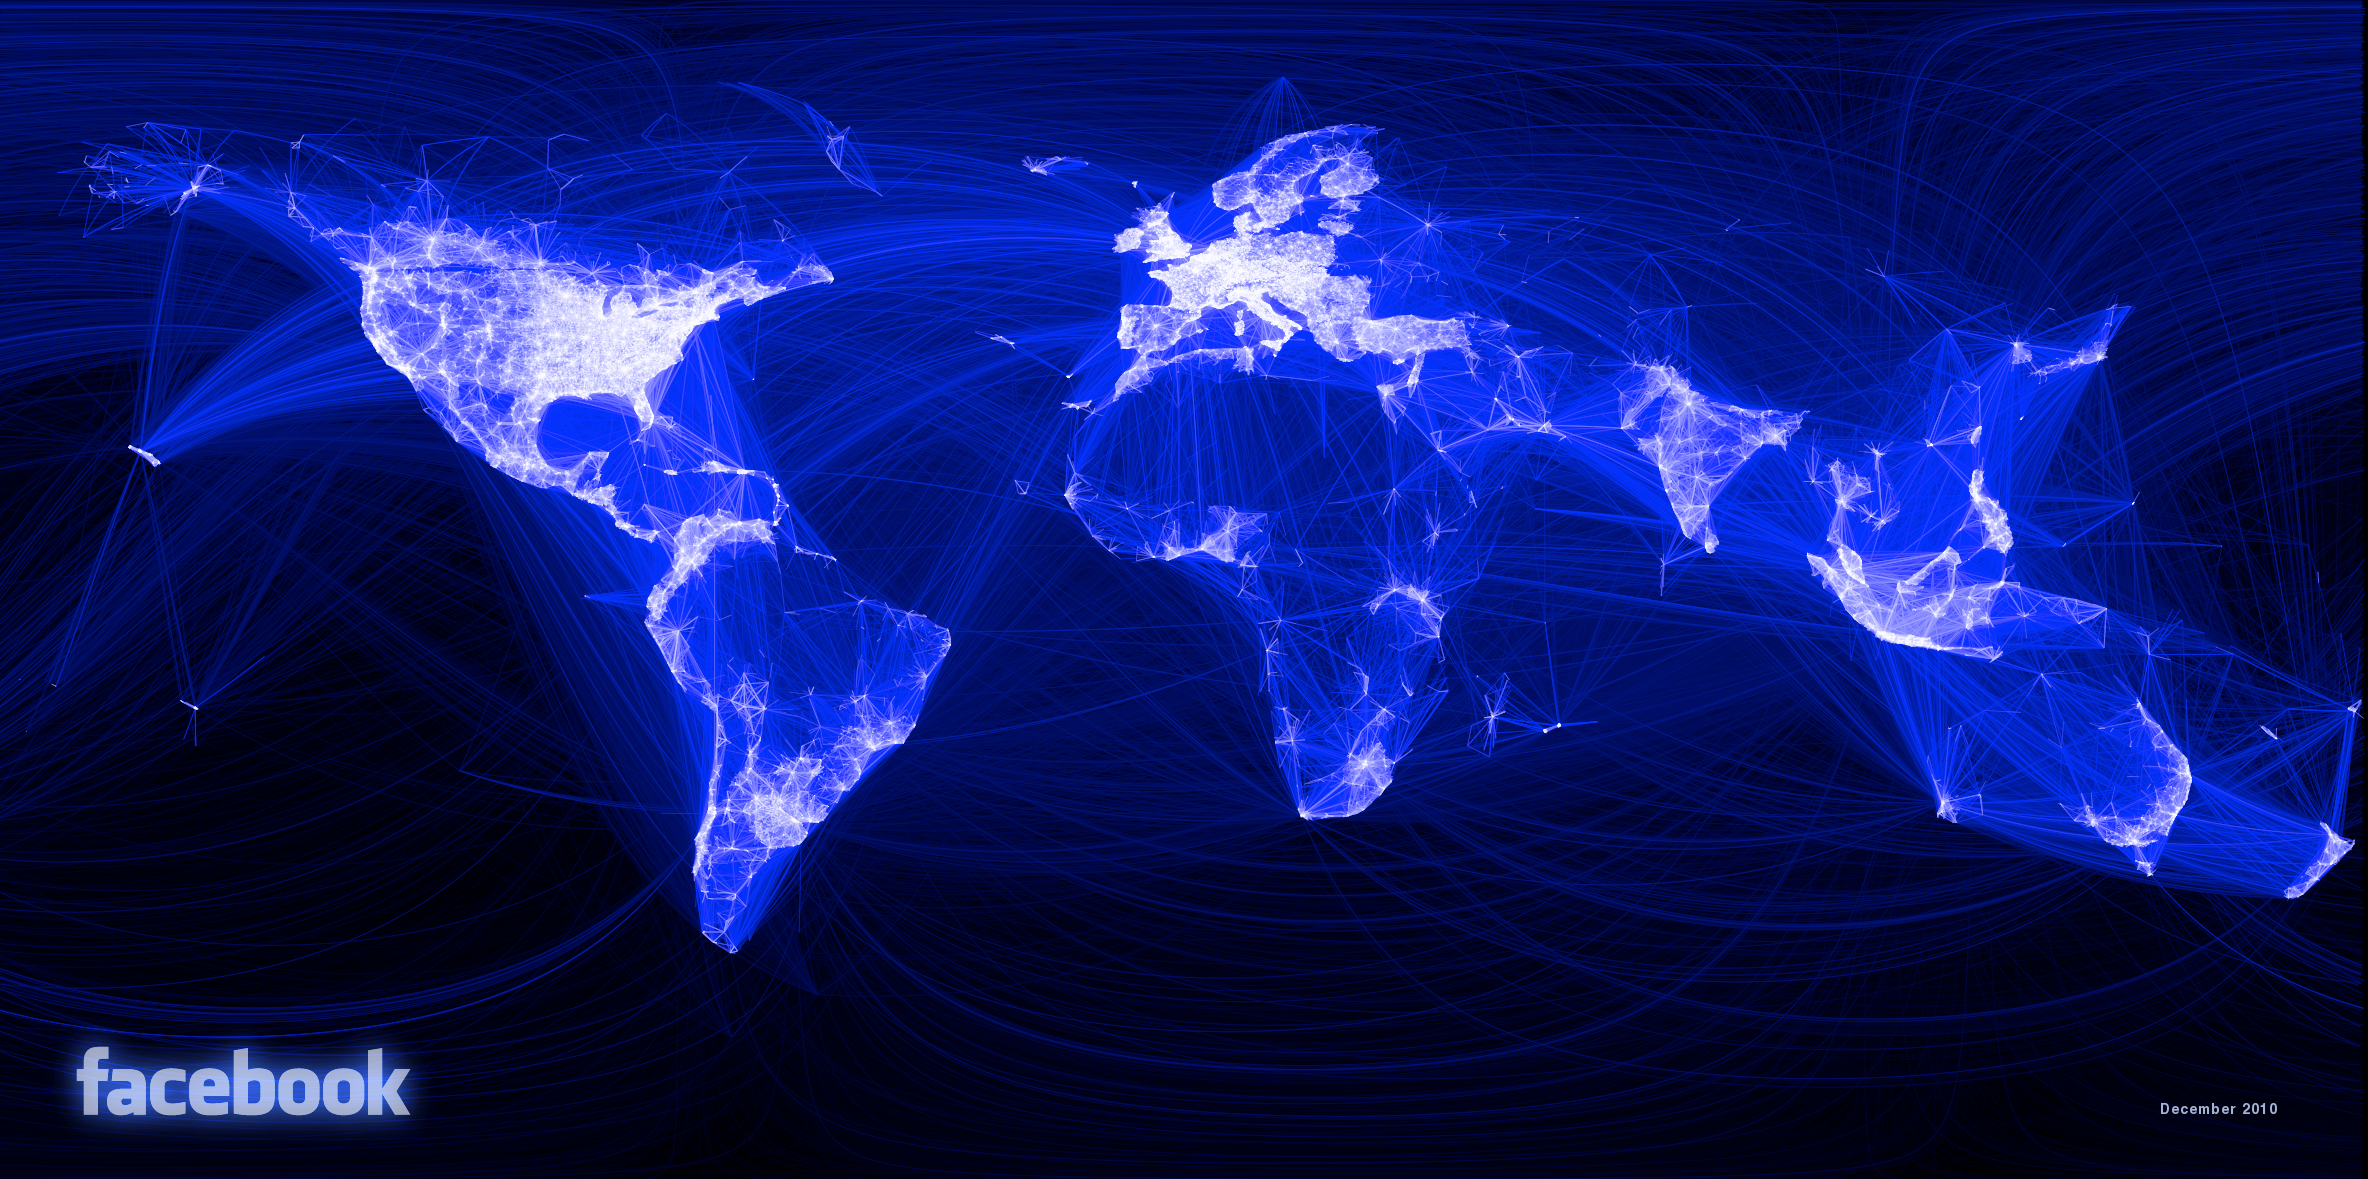
\includegraphics[scale=0.13]{images/facebook.png}
\end{center}
\vspace{-1em}
\begin{itemize}
\item Расчет PageRank всех страниц в интернете
\item Поиск по друзьям в социальной сети
\end{itemize}

\end{frame}

% ============================================== %

\begin{frame}{Суперкомпьютер VS кластер}

Проблемы
\begin{itemize}
\item данные не помещаются на HDD одной машины 
\item чтение со скоростью порядка сотен MB/s
\end{itemize}

Решения
\begin{itemize}
\item Супрекомпьютер \\
{\it много процессоров, специальное железо}
\item Кластер \\
{\it много ``обычных'' машин, соединенных сетью}
\end{itemize}

\end{frame}

% ============================================== %

\begin{frame}{Архитектура кластера}

\begin{center}
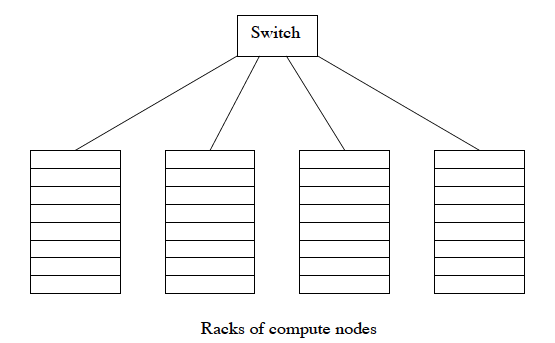
\includegraphics[scale=0.4]{images/cluster.png}
\end{center}

\begin{itemize}
\item Dual-processor x86, 2-4 GB, Linux machines
\item 1Gb/s Network switches
\item Inexpensive IDE disks
\end{itemize}

\end{frame}

% ============================================== %

\begin{frame}{Многое может пойти не так...}

\begin{itemize}
\item[DFS] Хранить несколько реплик данных
\item[MR] Вычисления нужно разбивать на части
\end{itemize}

\begin{center}

\includegraphics[scale=0.35]{images/fail.jpg}
\end{center}

\end{frame}

% ============================================== %

\section{(H)DFS}

% ============================================== %

\begin{frame}{Реализации DFS}

Примеры
\begin{itemize}
\item The Google File System (GFS)
\item Hadoop Distributed File System (HDFS)
\item CloudStore DFS by Kosmix
\end{itemize}

Свойства
\begin{itemize}
\item Файлы могут быть огромного размера
\item Данные не меняются, только добавляются
\item Файлы хранятся кусками (chunks)
\end{itemize}

\end{frame}

% ============================================== %

\begin{frame}{HDFS}

{\color{red} HDFS -- не файловая система общего назначения}
\begin{itemize}
\item Создана для хранения огромных массивов данных (Петабайты)
\item Предоставляет {\it надежный} доступ к данным
\item Поддерживает горизонтальное масштабирование
\item Хорошо интегрирована с Hadoop MapReduce
\end{itemize}

\end{frame}

% ============================================== %

\begin{frame}{Архитектура HDFS}

\vspace{-2em}
\begin{center}
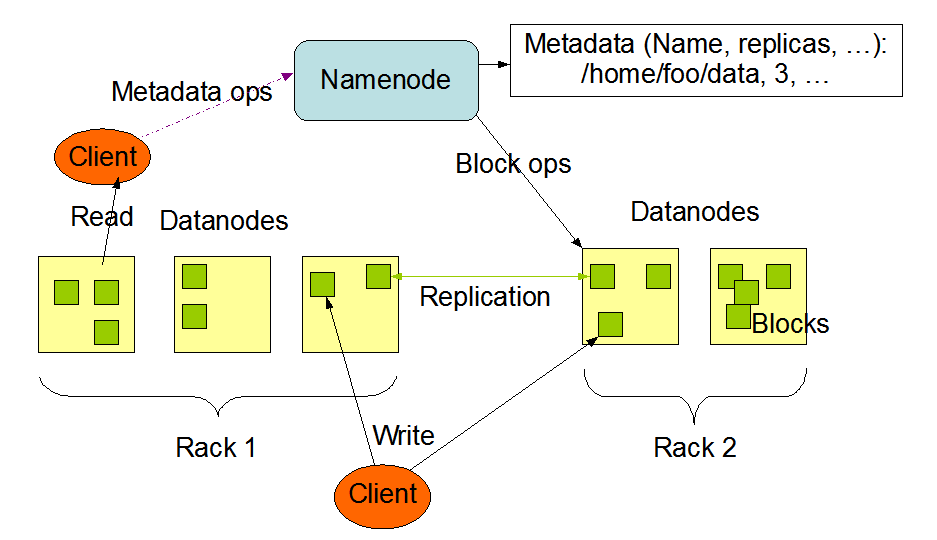
\includegraphics[scale=0.3]{images/hdfs.png}
\end{center}
\vspace{-2em}
\begin{itemize}
\item файлы хранятся блоками на Data Node \\ {\it по умолчанию 64М} 
\item метаданные хранятся в RAM на Name Node \\ {\it имя, права, расположение блоков на Data Node}
\end{itemize}

\end{frame}

% ============================================== %

\begin{frame}[fragile]{Доступ к файлам в HDFS}

Команды HDFS \url{http://hadoop.apache.org/docs/r0.18.3/hdfs_shell.html}

\begin{small}
\begin{shaded}
{\color{green} \begin{verbatim}
$ cat sample.txt 
A	12
B	12
A	14
A	22
C	12
$ hadoop fs -put sample.txt /user/anokhin
$ hadoop fs -ls /user/anokhin
\end{verbatim}}
\end{shaded}
\end{small}

Команды: \texttt{cat, cp, mv, rm, ls, put, get,...}(см документацию)

\end{frame}

% ============================================== %

\begin{frame}[fragile]{Подключение к кластеру Hadoop}

Для Windows \\ {\it скачиваем putty, подключаемся к \texttt{sfera-ds.openrise.org}}

\vspace{1em}
Для других ОС \\ {\it \texttt{ssh username$@$sfera-ds.openrise.org}}

\vspace{1em}
Пользователи
\begin{columns}[T]
    \begin{column}{.3\textwidth} 
	\begin{itemize}
\item alibekov
\item blagoveschenskiy
\item filipenko
\item kemaev
\item koltsov
\item kondratiev
\end{itemize}
    \end{column}
    \begin{column}{.3\textwidth} 
\begin{itemize}
\item kulikov
\item kulpinov
\item ludovichenko
\item medvedev
\item melnikov
\item mozharova
\end{itemize}    
    \end{column}
    \begin{column}{.3\textwidth} 
\begin{itemize}
\item nikolaev
\item novikov
\item ovlasuk
\item shvets
\item sovetov
\item taraban
\end{itemize}    
    \end{column}
\end{columns}

\end{frame}

% ============================================== %

\begin{frame}[fragile]{Данные}

\vspace{-0.5em}
Данные об активности пользователей в интернете за апрель 2014 находятся в директороии HDFS \texttt{/data/logs}
\begin{small}
\begin{shaded}
{\color{green} \begin{verbatim}
$ hadoop fs -cat /data/logs/20140425/part-00008 | head -5
\end{verbatim}}
\end{shaded}

\vspace{-1.5em}
\begin{center}
\begin{tabular}{l c c c}
\bf N & \bf Название & \bf Описание & \bf Пример \\
\hline
1 & $user\_id$ & ID пользователя & 100034b5 \\
2 & $timestamp$ & Unix time (сек) & 1398409877 \\
3 & $gender$ & 0 -- муж. 1 -- жен. & 1 \\
4 & $age$ & кол-во полных лет & 26 \\
5 & $os$ & oперационная система & win/win-xp \\
6 & $browser$ & браузер и версия & chrome/chrome-34 \\ 
7 & $resolution$ & разрешение экрана & 4 \\
8 & $touch$ & наличие тачскрин & 1 \\
9 & $hit\_url$ & URL посещенной страницы & https://e.mail.ru/ \\
10 & $referrer\_url$ & URL-referrer & http://mail.ru \\
11 & $load\_start$ & время начала загрузки & 1398065613566 \\
12 & $load\_end$ & время окончания загрузки & 1398065613590 \\
\end{tabular}
\end{center}
\end{small}

\end{frame}

% ============================================== %

\begin{frame}[fragile]{}

\begin{alertblock}{Вопрос 2 (1)}
Найти $user\_id$ последней записи в файле
\begin{shaded}
{\color{green} \begin{verbatim}
/data/logs/20140421/part-00008
\end{verbatim}}
\end{shaded}
\end{alertblock}

\end{frame}

% ============================================== %

\begin{frame}[fragile]{}

\begin{alertblock}{Вопрос 3 (1)}
Найти $referrer\_url$ четвертой записи в файле
\begin{shaded}
{\color{green} \begin{verbatim}
/data/logs/20140421/part-00000
\end{verbatim}}
\end{shaded}
Подсказка: head
\end{alertblock}

\end{frame}

% ============================================== %

\begin{frame}[fragile]{}

\begin{alertblock}{Вопрос 4 (1)}
Посчитать количество записей в файле
\begin{shaded}
{\color{green} \begin{verbatim}
/data/logs/20140421/part-00000
\end{verbatim}}
\end{shaded}
Подсказка: wc -l
\end{alertblock}

\end{frame}

% ============================================== %

\begin{frame}[fragile]{}

\begin{alertblock}{Вопрос 5 (2)}
Посчитать количество записей, сделанных мужчинами и женщинами в файле
\begin{shaded}
{\color{green} \begin{verbatim}
/data/logs/20140421/part-00000
\end{verbatim}}
\end{shaded}
Подсказка: sort, uniq, cut
\end{alertblock}

\end{frame}

% ============================================== %

\begin{frame}[fragile]{}

\begin{alertblock}{Вопрос 6 (2)}
Вывести список $user_id$[tab]$age$ из 10 самых старых пользователей в файле
\begin{shaded}
{\color{green} \begin{verbatim}
/data/logs/20140421/part-00000
\end{verbatim}}
\end{shaded}
Подсказка: sort, cut, head
\end{alertblock}

\end{frame}

% ============================================== %

\section{MapReduce}

% ============================================== %

\begin{frame}{Идея MapReduce}

{Цель -- обработка больших объемов данных параллельно на нескольких машинах}

\begin{center}
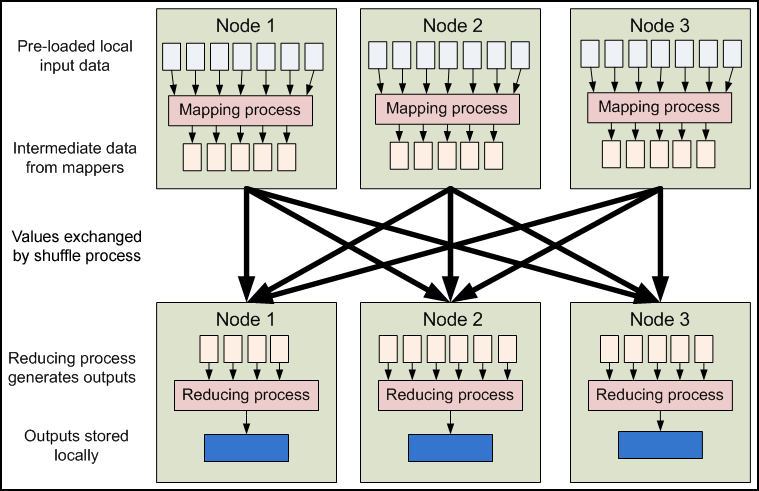
\includegraphics[scale=0.33]{images/mr.png}
\end{center}

\end{frame}

% ============================================== %

\begin{frame}{Map}

Из исходного файла последовательно считываются пары ключ-значение и подаются в функцию {\bf map}

\begin{center}
Сигнутура: \texttt{($k_1$, $v_1$) $\rightarrow$ list($k_2$, $v_2$) }

\vspace{2em}

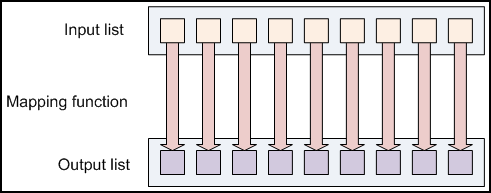
\includegraphics[scale=0.33]{images/map.png}
\end{center}

\end{frame}

% ============================================== %

\begin{frame}{Reduce}

Все значения, принадлежащие одному ключу, обрабатываются функцией {\bf reduce}

\begin{center}
Сигнутура: \texttt{($k_2$, list($v_2$)) $\rightarrow$ list($k_2$, $v_2$) }

\vspace{2em}

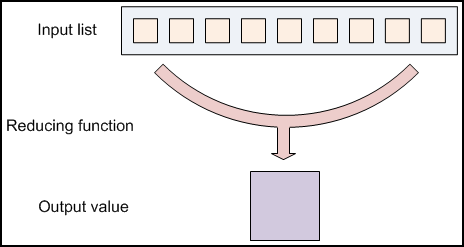
\includegraphics[scale=0.33]{images/reduce.png}
\end{center}

\end{frame}

% ============================================== %

\begin{frame}{Умножение матрицы на вектор}

\begin{block}{Пример}
Дана матрица  $M$ размера $n \times n$ с элементами $m_{ij}$ и вектор $v$ с элементами $v_j$.  
\end{block}

Расмотрим случаи
\begin{enumerate}
\item $v$ помещается в память одной машины
\item $v$ не помещается в память одной машины
\end{enumerate}

\end{frame}

% ============================================== %

\begin{frame}{MapReduce на Hadoop}

\vspace{-1em}
\begin{center}
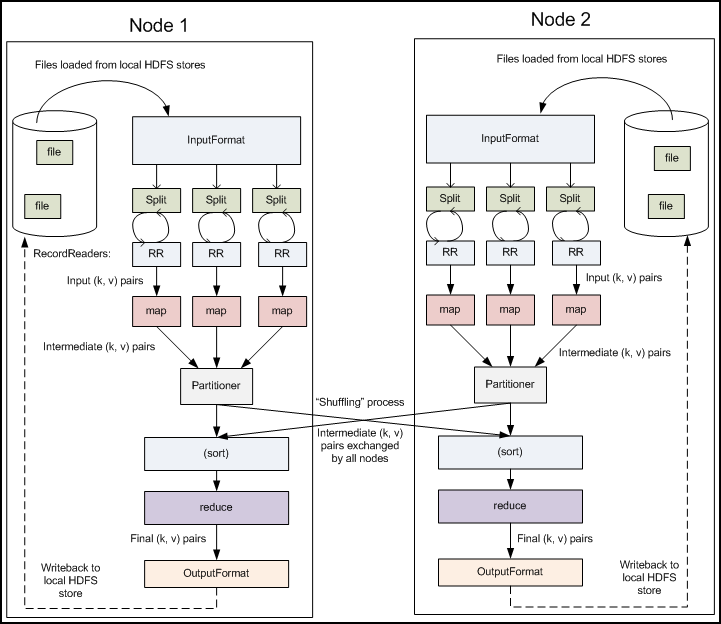
\includegraphics[scale=0.33]{images/hmr.png}
\end{center}

\end{frame}

% ============================================== %

\begin{frame}{Combine}

Пусть {\bf reduce} -- коммутативен и ассоциативен

\begin{center}
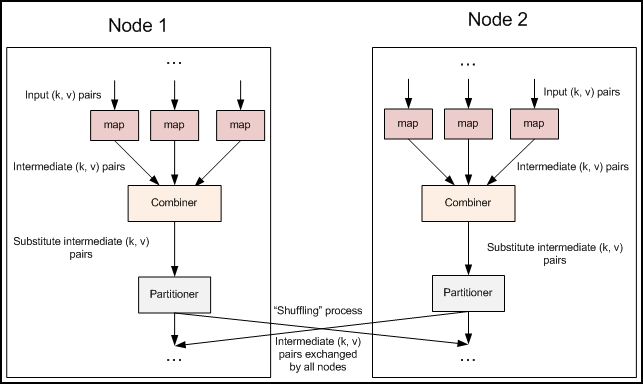
\includegraphics[scale=0.33]{images/combine.png}
\end{center}

\end{frame}

% ============================================== %

\begin{frame}{Когда что-то все-же пошло те так}

\begin{itemize}
\item[П1] Недоступна машина, выполняющая Reduce \\
{\it другие машины выполняют заново {\bf не законченные} ей задачи}
\item [П2] Недоступна машина, выполняющая Map \\
{\it другие машины выполняют заново {\bf все} ее задачи}
\end{itemize}

Вывод: минимизировать коммуникацию между машинами

\end{frame}

% ============================================== %

\begin{frame}{Операторы реляционной алгебры}

\begin{itemize}
\item[S] Selection с условием $C$: $\sigma_C(R)$
\item[P] Projection на подмножество $S$: $\pi_S(R)$
\item[J] Natural Join: $R \Join S$
\item[U] Union (intersection, difference): $R \cup S$
\item[G] Grouping аттрибутами $X$: $\gamma_X(R)$
\end{itemize}

\end{frame}

% ============================================== %

\begin{frame}{Hadoop экосистема}

\begin{columns}[T]
    \begin{column}{.4\textwidth} 
	\begin{itemize}
\item Hadoop (MapReduce)
\item Hive (SQL-like via MR)
\item Pig (язык запросов для Hadoop)
\end{itemize}
    \end{column}
    \begin{column}{.6\textwidth} 
\begin{itemize}
\item Mahout (ML)
\item Spark (SQL + ML + Graphs + Streaming)
\item Tez (ациклические workflow)
\end{itemize}    
    \end{column}
\end{columns}

\begin{center}
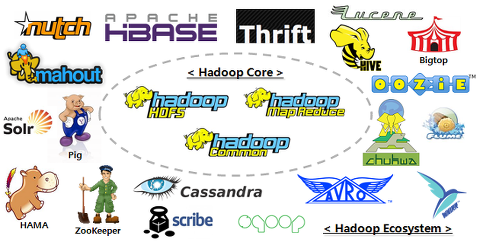
\includegraphics[scale=0.55]{images/eco.png}
\end{center}

\end{frame}

% ============================================== %

\begin{frame}[fragile]{}

\begin{alertblock}{Вопрос 8 (3)}
Реализовать Hadoop job для вычисления количества посещений на каждом из доменов. Распечатать список из 20 самых посещаемых доменов 15 апреля (вместе с количеством посещений).
\end{alertblock}

\begin{alertblock}{Вопрос 9 (3)}
Построить график распределения количества посещений доменов в натуральной шкале и в логарифмической по обоим осям.
\end{alertblock}

\end{frame}

\end{document}